\documentclass[10pt]{article}

\usepackage[margin=1in]{geometry}
\usepackage{float,glossaries,graphicx,hyperref}

\makenoidxglossaries

\newglossaryentry{Binary Separated Value}
{
    name=Binary Separated Value,
    description={The filetype associated with the encoding protocols laid out in this document}
}

\newglossaryentry{.bsvx}
{
    name=.bsvx,
    description={The file extension associated with the Binary Separated Value file format}
}

\newglossaryentry{.csv}
{
    name=.csv,
    description={Comma-separated values file format often used for databases and spreadsheets}
}

\newglossaryentry{.tsv}
{
    name=.tsv,
    description={Tab-separated values file format used for databases and spreadsheets}
}

\newglossaryentry{Comma delimiter}
{
    name=Comma delimiter,
    description={Practice of using the ‘,’ character as a field separator to differentiate records in a file. Instances of a comma are always interpreted as a delimiter unless they appear in doubles quotes e.g. “1,0”}
}

\newglossaryentry{Serialization}
{
    name=Serialization,
    description={The process of encoding an object as a .bsvx format byte stream}
}

\newglossaryentry{Deserialization}
{
    name=Deserialization,
    description={The process of decoding of a .bsvx byte stream and reconstruction of the original data}
}

\newglossaryentry{Libre Calc}
{
    name=Libre Calc,
    description={An open-source application for manipulating spreadsheets. Developed and maintained by The Document Foundation}
}

\begin{document}

\title{Binary Separated Value\\Architecture}
\author{B. Bean, N. Mezher, J. Summers \& D. Toomey\\University of Massachusetts Lowell | Software Engineering II\\Prof. James Daly}
\date{February 2020}
\maketitle

\section*{Motivation}

The use of databases as a means for storing information has become ubiquitous in every field concerning data.
One of the most common methods for analyzing sets of data from databases is to export it to a \texttt{.csv} file in order to manipulate the data via a spreadsheet program or language libraries.
But despite all its draws, the \texttt{.csv} format has some significant drawbacks as well.
The format is too bulky and inefficient for many applications, and it relies on a comma delimiter to separate data which can be problematic \cite{Coleman2011}.
Our improvements upon the \texttt{.csv} format will allow for users and programs to more efficiently store and utilize complex data.
The end goal is to expedite communication between programs and disparate systems.

\indent{}
This document will outline the proposal of a new format called Binary Separated Value (\texttt{.bsvx}).
This format of data will be delimited with byte markers which begin each field telling the library what kind of data will be in the field and how long it will be.
Instead of using a character delimitation in plaintext form, using a byte marker solves the issue of having commas in string fields, avoiding parsing errors.
One drawback of this style of implementation is the inability to parse and edit \texttt{.bsvx} files through a text editor, but this issue is remedied through the BSVX LibreOffice Calc Extension.
The Binary Separated Value format will be processed through a proprietary Python library.

\indent{}
LibreOffice is a free to use, open-source file editing platform similar to Microsoft Office.
Calc is a program provided in the LibreOffice suite, and provides similar functionality to Microsoft’s Excel program \cite{Guthrie2012}.
The proposed BSVX Calc Extension will give Calc users the ability to read data from a \texttt{.bsvx} file, and export their spreadsheets in \texttt{.bsvx} format.
This will also allow users the functionality of converting a \texttt{.csv} file into a \texttt{.bsvx} file through the Calc program.

\section*{BSVX File Type Specification}

Each \texttt{.bsvx} file contains a series of rows of headers or records.
Each row begins with a byte marker denoting the type (i.e. header or record) and the number of fields within that row.
Following the first byte marker of a row is a series of fields, each made up of two parts: a byte marker denoting the type and size of the data stored within the field, and the data itself.
Some initial markers will indicate that the size of the data will be given in subsequent bytes.
Once the length \textit{n} is determined, those \textit{n} bytes can be interpreted to match the field byte marker.
Each row does not have to be the same length, the data can be jagged and parsers will only read as much data as is denoted by the first byte marker of each row. 

\indent{}
At any time, the parser knows how many bytes it needs to read.
There will never be an instance where it needs to read bytes until it sees a particular byte (like in the case of \texttt{.csv} or \texttt{.tsv} looking for a comma or tab to end on).
Strings will neither need end marks nor escape characters, and will be stored in UTF-8 format.
The byte marker for strings denotes the number of bytes read, not the number of characters of the string itself.
All numbers are stored in little endian order.

\indent{}
An abstract example of a \texttt{.bsvx} file row (header or record) looks like this:

\begin{table}[H]
\centering
\begin{tabular}{|c|c|c|c|c|c|c|}
\hline
3 & 3 & FOO & 2 & 1000 & 4 & 25.345 \\
Field & str &  & int &  & Float &  \\ \hline
\end{tabular}
\caption{An example of a \texttt{.bsvx} file row.}
\label{tab:bsvxApproach_example}
\end{table}

\indent{}
The following table will be used to implement each type of supported data in its own class and denote the bit range each field will be denoted by, ranging from 0 to 255.
The first column gives the parser crucial context: what type of data will follow the byte marker, and further, which \textit{variant} on that type it will be.
For example, the small integer (int) type is represented by numbers in the range 136-143. 
A 2-byte small int is indicated by 138, 139 is for a 3 byte int, 140 denotes a 4 byte int, etc.
The second column illustrates how the range of values for a given type is affected by the magnitude of its offset i.e. for a small int, the second column entry is 136 + [0, 7].
The third column establishes the types of data that are supported and the fourth provides a brief description of each.

\begin{table}[H]
\centering
\resizebox{\textwidth}{!}{%
\begin{tabular}{|c|c|c|l|}
\hline
\textbf{Range} & \textbf{Form} & \textbf{Name} & \textbf{Description} \\ \hline
0 &  & Blank & Possible implementation: NULL or ‘empty string’ \\ \hline
1-127 & 1-127 & Short str & UTF-8 Encoded string of byte length 1-127 \\ \hline
128-135 & 128 + {[}0,7{]} & Long str & 1-8 bytes giving the length of a str, followed by said str \\ \hline
136-143 & 136 + {[}0,7{]} & Small int & An integer in the range of 0-7 bytes \\ \hline
144-151 & 144 + {[}0,7{]} & Long int & A zig-zag encoded integer using 1-8 bytes \\ \hline
152-159 & 152 + {[}0,7{]} & Float & IEEE-754 format float: 0 = half precision, 1 = single, 2 = double, 3 = triple \\ \hline
160-167 & 160 + {[}0,7{]} & Blob & 1-8 bytes giving the length of binary data in bytes, followed by said data \\ \hline
168-183 & 168 + {[}0,15{]} & Header & Beginning of header with 0-15 fields \\ \hline
184-191 & 184 + {[}0,7{]} & Long header & 1-8 bytes giving the number of fields in the header \\ \hline
192-207 & 192 + {[}0,15{]} & Record & Beginning of record with 0-15 fields \\ \hline
208-215 & 208 + {[}0,7{]} & Long record & 1-8 bytes giving the number of fields in the record \\ \hline
216-255 &  & Reserved & For future use \\ \hline
\end{tabular}%
}
\caption{Data types supported by the BSVX file type specification.}
\label{tab:bsvxApproach_dataTypes}
\end{table}

\section*{Deliverables}

The proposed deliverables for this new format include a LibreOffice Calc extension to read from and write to \texttt{.bsvx} files, and a Python library for doing the same.
This extension should be capable of converting between \texttt{.csv} and \texttt{.bsvx} without loss or adulteration of the information stored in the files.
Similar libraries for languages such as Java, C++ and C\#, or JavaScript are left as stretch goals.

\indent{}
The BSVX Calc Extension will allow spreadsheets to be saved to and read from \texttt{.bsvx} files.
To illustrate the top-most point for user interaction with the BSVX Calc Extension, there is included a series of figures below. 
\autoref{fig:deliverables_mockupPart1} displays the default toolbar packaged with LibreOffice Calc.
\autoref{fig:deliverables_mockupPart2} contrasts the differences between the default toolbar and the toolbar with the BSVX Calc Extension enabled.
It can be seen that only two features are added, in the form of two buttons.
The proposed left button allows for importing, reading from, a \texttt{.bsvx} file and the proposed right button for exporting, saving to, a \texttt{.bsvx} file.
Finally, \autoref{fig:deliverables_mockupPart3} provides a glance as to how the toolbar will look with the BSVX Calc Extension enabled.

\begin{figure}[H]
\centering
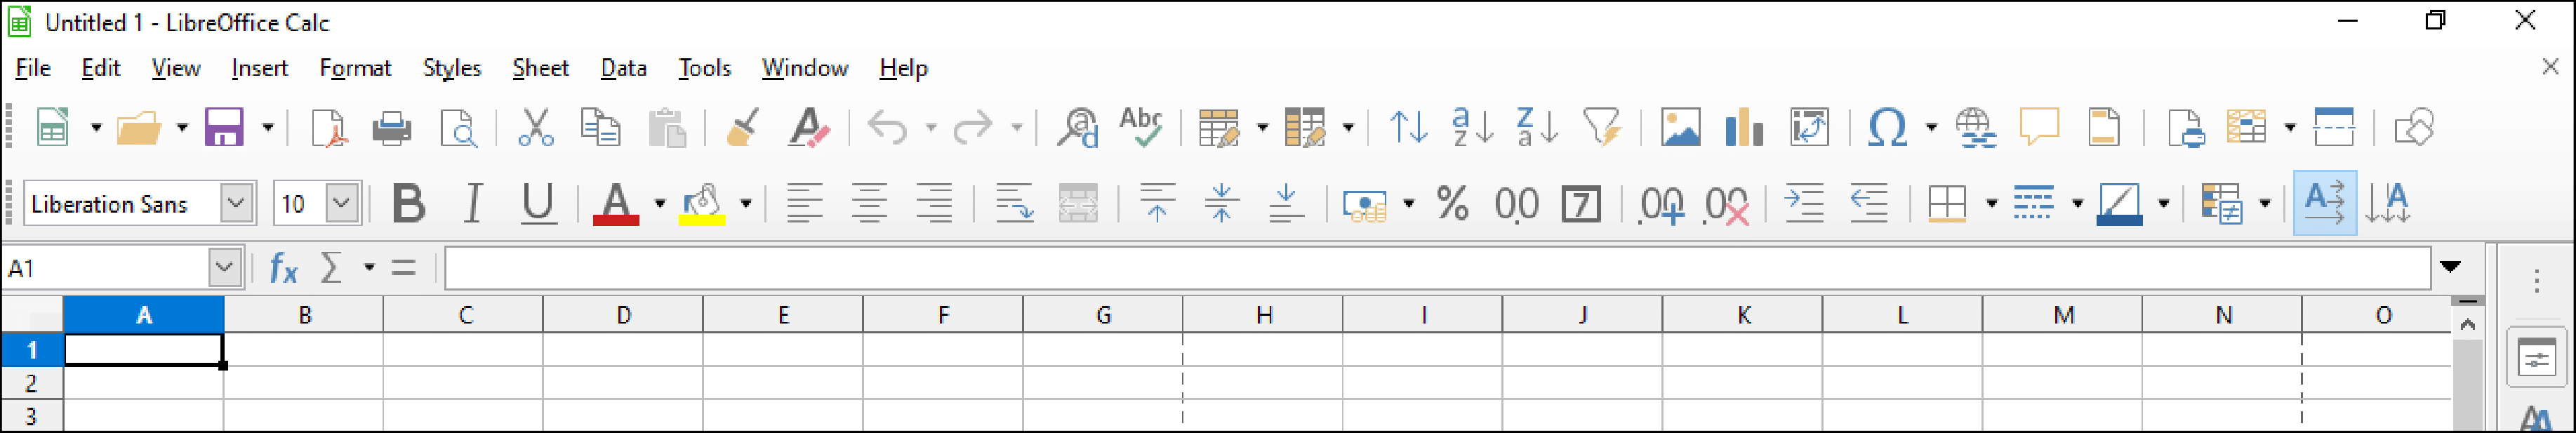
\includegraphics[width=\textwidth]{figures/mockupPart1.png}
\caption{LibreOffice Calc's toolbar.}
\label{fig:deliverables_mockupPart1}
\end{figure}

\begin{figure}[H]
\centering
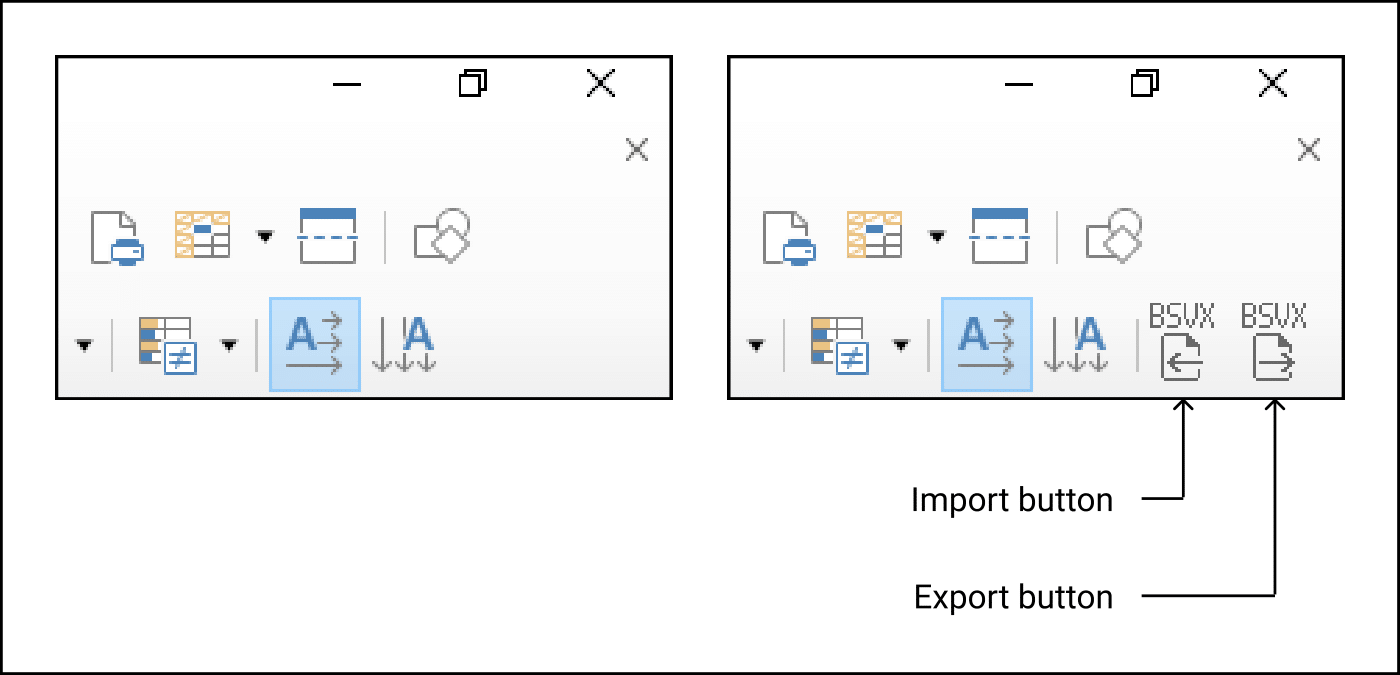
\includegraphics[width=4in]{figures/mockupPart2.png}
\caption{The BSVX Calc Extension will provide two additional buttons for importing and exporting.}
\label{fig:deliverables_mockupPart2}
\end{figure}

\begin{figure}[H]
\centering
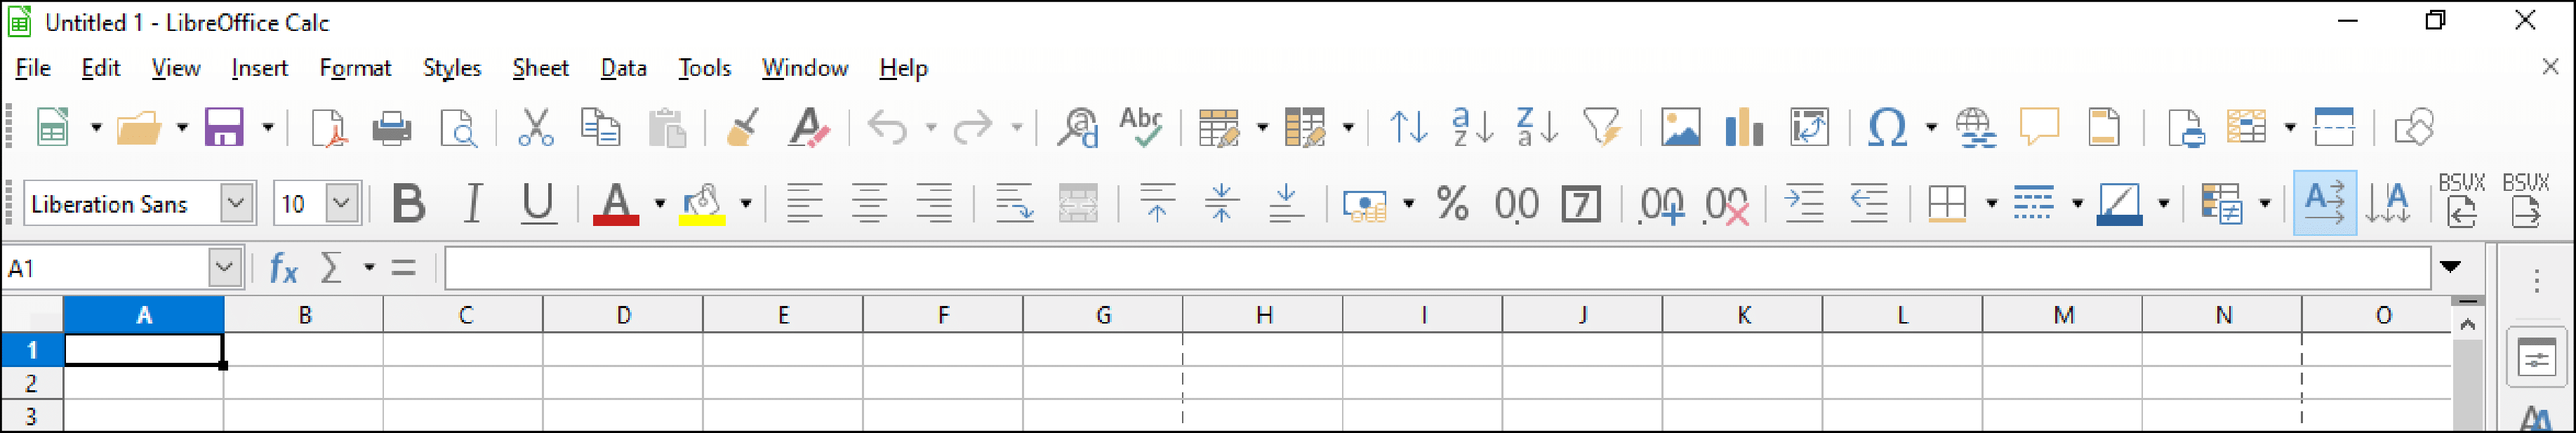
\includegraphics[width=\textwidth]{figures/mockupPart3.png}
\caption{A mockup of LibreOffice Calc's toolbar with the BSVX Calc Extension enabled.}
\label{fig:deliverables_mockupPart3}
\end{figure}

\indent{}
To talk more about how the BSVX Calc Extension works behind the scenes, it is first necessary to speak about our proposed Python library---\texttt{bsvxpy}.
As a generality, our Python library will be similar to the \texttt{.csv} library.
A writer function will be passed a series of fields representing a header row. 
Subsequent binary values are decoded based on the corresponding type casts provided by the header.
The library will then extract each of the fields from the dictionary object and output them to the Calc spreadsheet in sequential order.
The library will also process nested data structures within the \texttt{.bsvx} file allowing for the recursive encoding and decoding of further dictionary objects.

\begin{figure}[H]
\centering
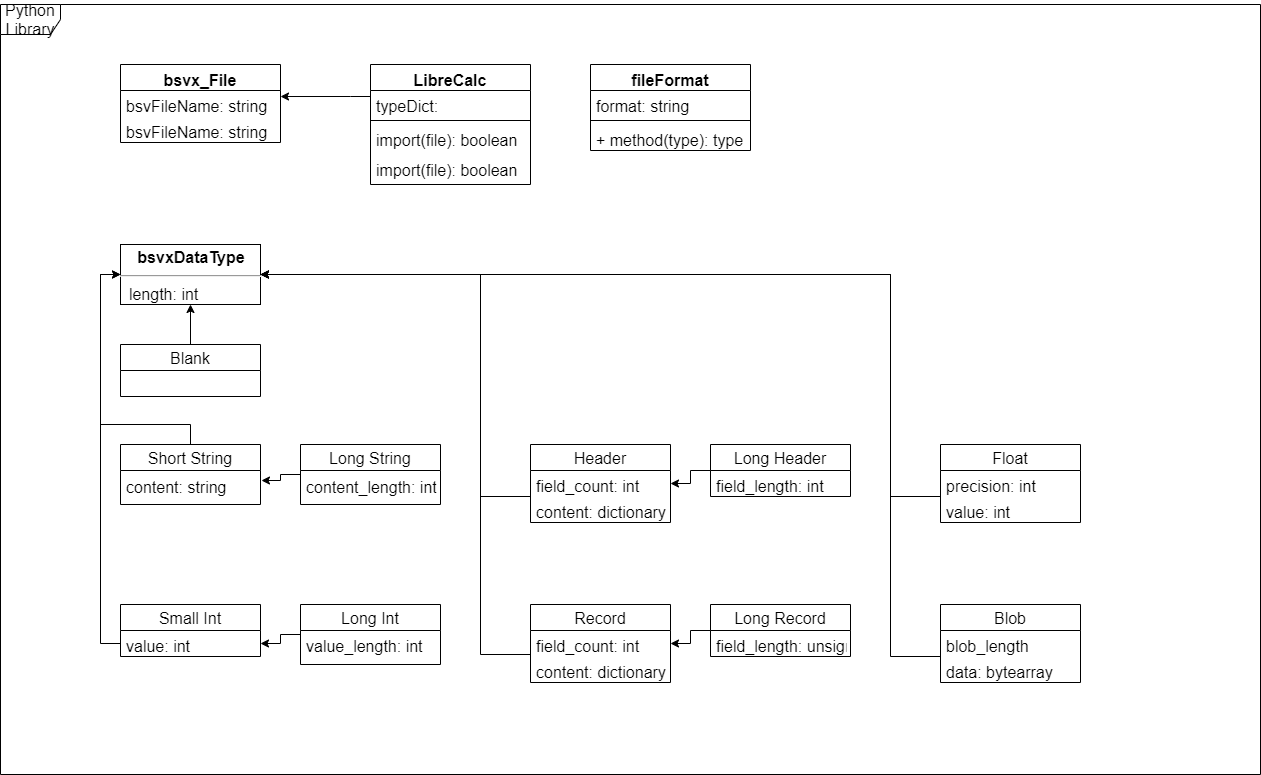
\includegraphics[width=\textwidth]{figures/bsvxpy.png}
\caption{UML diagram outlining the classes and statstructures used in bsvxpy}
\label{fig:bsvxpy_architecture}
\end{figure}


\indent{}
With an understanding of how the \texttt{bsvxpy} Python library functions, we can return to an overview of the BSVX Calc Extension.
First off, the LibreOffice Calc project allows developers to create extensions using Python, which lets us extend LibreOffice Calc’s functionality to include \texttt{.bsvx} file support using our \texttt{bsvxpy} Python library.
We will also be using the \texttt{uno} Python library, as it is necessary for any LibreOffice Calc extension development.

\indent{}
To export data to a \texttt{.bsvx} file, the BSVX Calc Extension will call functions from the \texttt{uno} Python library to read cell data from LibreOffice Calc.
The \texttt{bsvxpy} Python library will then be used to convert that data into binary separated values.
Once the data is appropriately converted, it will be written to a file---as named by the user---with the file extension \texttt{.bsvx}.
\autoref{fig:deliverables_dataToBsvx} depicts the data flow for the exporting feature.

\begin{figure}[H]
\centering
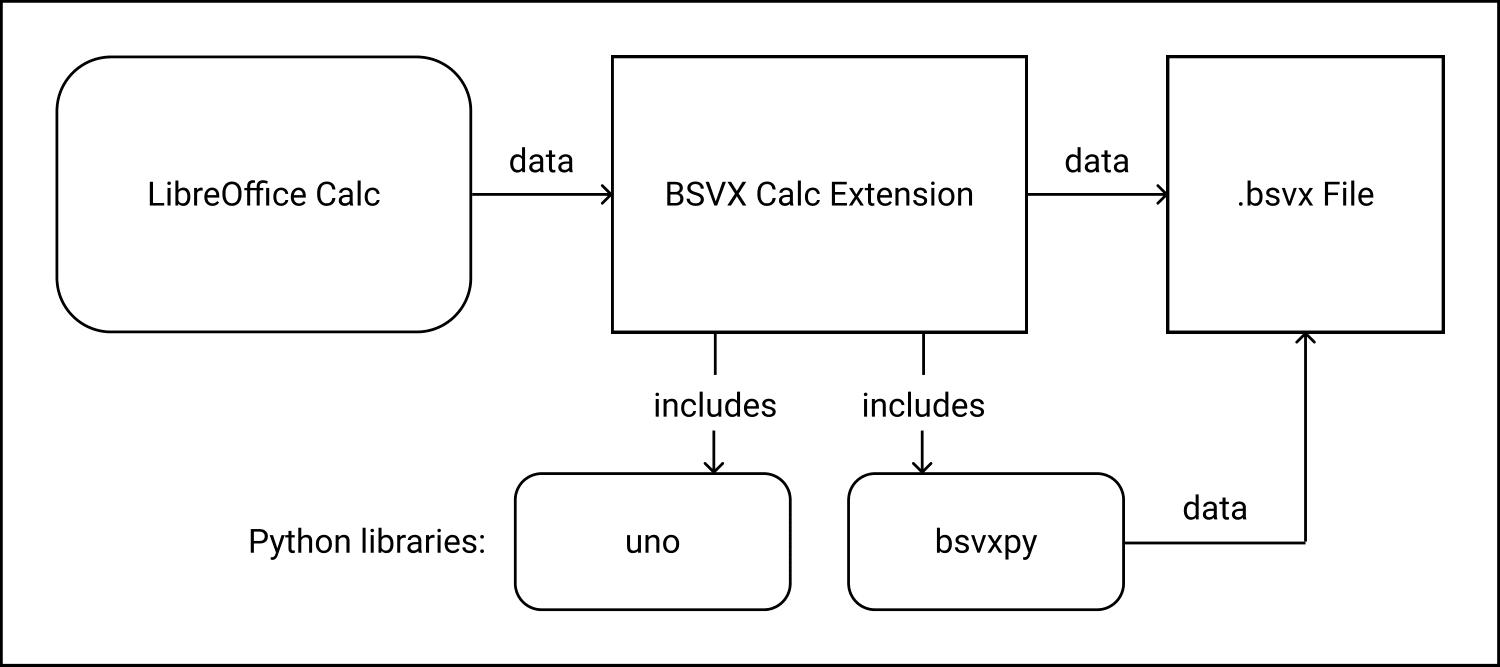
\includegraphics[width=5in]{figures/dataToBsvx.png}
\caption{Scope of API and library calls for the BSVX Calc Extension in exporting data to a \texttt{.bsvx} file.}
\label{fig:deliverables_dataToBsvx}
\end{figure}
\newpage

\indent{}
The importing feature works the same way, but in reverse.
The user selects a \texttt{.bsvx} file to import data from, and the BSVX Calc Extension reads data from that file, using \texttt{bsvxpy} and \texttt{uno} to translate it from binary separated value data to cell data that LibreOffice Calc can read.
The data flow for the importing feature is represented by \autoref{fig:deliverables_bsvxToData}.
    
\begin{figure}[H]
\centering
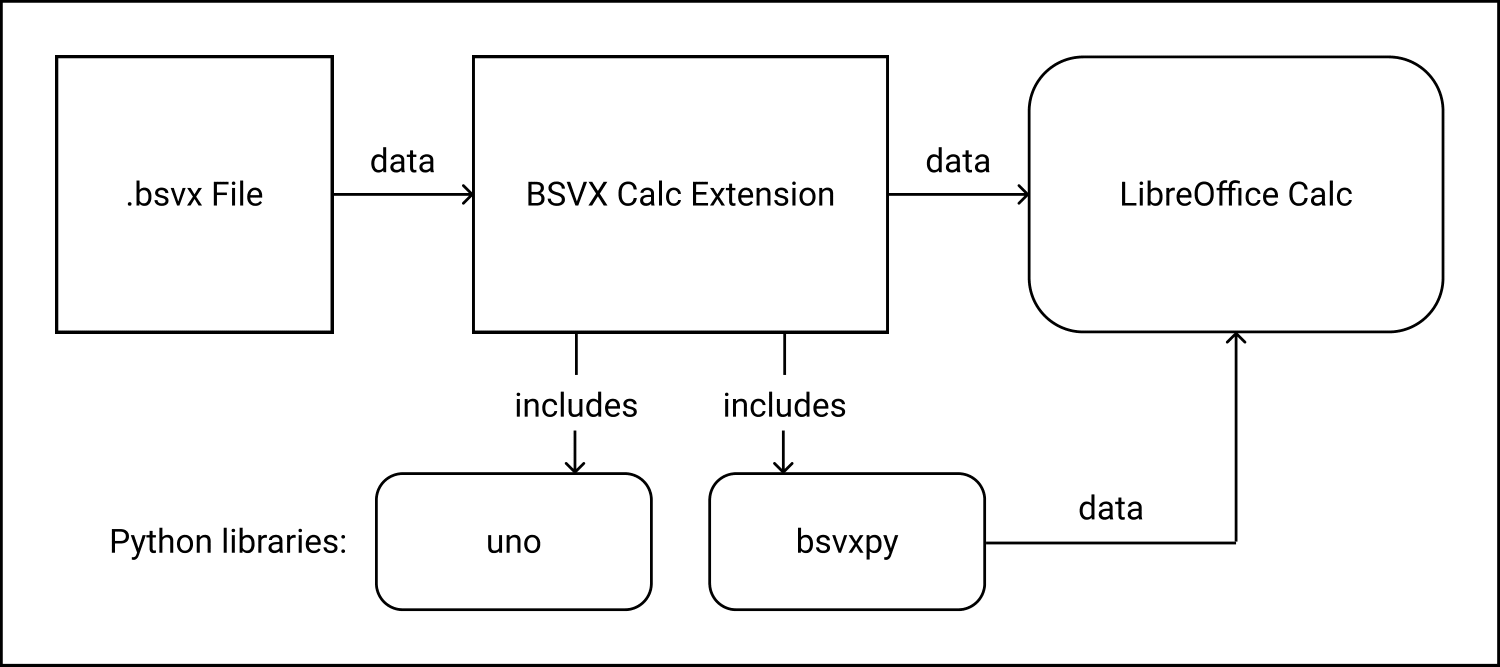
\includegraphics[width=5in]{figures/bsvxToData.png}
\caption{Scope of API and library calls for the BSVX Calc Extension in importing data from a \texttt{.bsvx} file.}
\label{fig:deliverables_bsvxToData}
\end{figure}

\indent{}
This functionality also allows the user to convert from \texttt{.csv} to \texttt{.bsvx}.
If the user chooses to import a \texttt{.csv} file into LibreOffice Calc, and exports that file to a \texttt{.bsvx} file, that same data will be available in both files.
Likewise, if the user chooses to import a \texttt{.bsvx} file and export that file to a \texttt{.csv} file, that same data will be available.
These changes do not significantly affect the overall architecture of LibreOffice Calc.
The same base functionality of LibreOffice Calc is still provided to the user once this extension is installed, with the addition of importing and exporting features for \texttt{.bsvx} file formats.

\section*{Approach}

As the specifications for the \texttt{.bsvx} file format have already been articulated, our main goal is to implement novel import/export functionality in Libre Calc.
Example \texttt{.bsvx} files will be manually created to accurately account for testing basic functionality as well as edge cases.
Initial builds will emphasize basic functionality such as correctly reading/writing basic data types, and will move to nested and blob types after initial testing is completed.
Lastly, we’ll attempt to optimize memory and computational efficiency to improve performance outcomes.

\indent{}
One important test of the \texttt{.bsvx} format and its corresponding extension will be its capacity to maintain full integrity of the data after conversion to and from \texttt{.csv} format.
Our deliverable should enable a user with minimal experience in LibreOffice and some experience with spreadsheets to perform these conversions without loss of data or corruption of its ordering.
Some loss of formatting and style is acceptable as long as the order of the values and the values themselves are maintained.
The point of \texttt{.bsvx} is not aesthetics, it is purely function.

\indent{}
The project is expected to approximately two months to complete, with production wrapping in late April 2020.
Costs are to be kept minimal, if nonexistent, as our developers are being paid in “experience.”

\section*{Schedule and Milestones}

\begin{table}[H]
\centering
\resizebox{\textwidth}{!}{%
\begin{tabular}{|l|l|}
\hline
\textbf{Date} & \textbf{Goal} \\ \hline
February 19, 2020 & Finish background research, draft Object and Interaction UML diagrams \\ \hline
February 26, 2020 & Finalize list of required development tools, testing environment, lock LibreOffice version for internal development \\
 & Decompose development steps and and assign tasks \\ \hline
March 4, 2020 & Finalize and submit our User Manual \\ \hline
March 6, 2020: Midterm Milesome & Draft LibreOffice Calc interface \\
 & Draft .bsvx interpreter with the expected functionality of converting .csv to .bsvx file type (one way) \\ \hline
March 18, 2020 & Finalize Calc interface \\
 & Draft .bsvx import functionality (.bsvx to .csv file type) \\ \hline
April 1, 2020 & Merge Calc interface and .bsvx interpreter with stretch goal of eliminating .csv middle-step \\ \hline
April 17, 2020 & Draft Final Report of findings \\ \hline
April 27, 2020: Final Milestone & Submit Final Report and Present findings to class \\ \hline
\end{tabular}%
}
\caption{Purported project schedule.}
\label{tab:approach_schedule}
\end{table}

\section*{Challenges and Risks}

One of the primary risks is the possibility that there are undiscovered ambiguities in the format specification.
These will be dealt with by tightening the specification to account for ambiguities, and updating the reference implementation.
Additionally, parsing \texttt{.csv} files for conversion to \texttt{.bsvx} files, and vice-versa, could involve numerous pitfalls.
While there is an agreed upon standard format for \texttt{.csv} files, it didn’t come about until 2005 and many \texttt{.csv} files still do not conform to it strictly.
This will complicate our attempt to ensure integrity and continuity between conversions for \textit{all} \texttt{.csv} and \texttt{.bsvx} files.
For instance, when converting a a \texttt{.bsvx} file consisting of several strings of comma characters, our library would have to ensure that none of the commas end up being misinterpreted as delimiters.
Properly following the specification will ensure consistency and prevent this from happening, but rigorous testing with a myriad of files will be necessary.

\indent{}
One challenge fundamental to the \texttt{.bsvx} format itself is deciding how to handle blob objects.
It isn’t always clear what type of data they should be deserialized as.
Perhaps Calc has a method to interpret unknown fields upon reading the file; more research will be done on this.
Another challenge is that the framework/API for both LibreOffice and Calc is unfamiliar, and it will take some time to learn.

\clearpage
\glsadd{Binary Separated Value}
\glsadd{.bsvx}
\glsadd{.csv}
\glsadd{.tsv}
\glsadd{Comma delimiter}
\glsadd{Serialization}
\glsadd{Deserialization}
\glsadd{Libre Calc}
\printnoidxglossary[nonumberlist]

\clearpage
\begin{thebibliography}{9}

  \bibitem{Coleman2011}
    Coleman, Larry.
    "Why do we keep using CSV?"
    Software Engineering Stack Exchange,
    14 Feb. 2011.
    \url{https://softwareengineering.stackexchange.com/questions/47838/why-do-we-keep-using-csv}

  \bibitem{"CSV File Reading and Writing"2020}
    “CSV File Reading and Writing.”
    Python Docs,
    12 Feb. 2020.
    \url{https://docs.python.org/3/library/csv.html}

  \bibitem{DalyMeiners2020}
    James Daly and Meiners, Chad.
    “Binary Separated Value.”
    UMass Lowell,
    30 Jan. 2020.

  \bibitem{Guthrie2012}
    Guthrie, Gordon.
    “How to Work With LibreOffice Calc.”
    TechRadar,
    23 July 2012.
    \url{https://www.techradar.com/news/world-of-tech/roundup/how-to-work-with-libreoffice-calc-1089870}
  
\end{thebibliography}

\end{document}
